\section{\begin{CJK}{UTF8}{gkai}
		MapReduce复现
\end{CJK}}

\subsection{\begin{CJK}{UTF8}{gkai}
		分布式MapReduce
\end{CJK}}

\begin{frame}{\begin{CJK}{UTF8}{gkai}主要机制
	\end{CJK}}
	
	\centerline{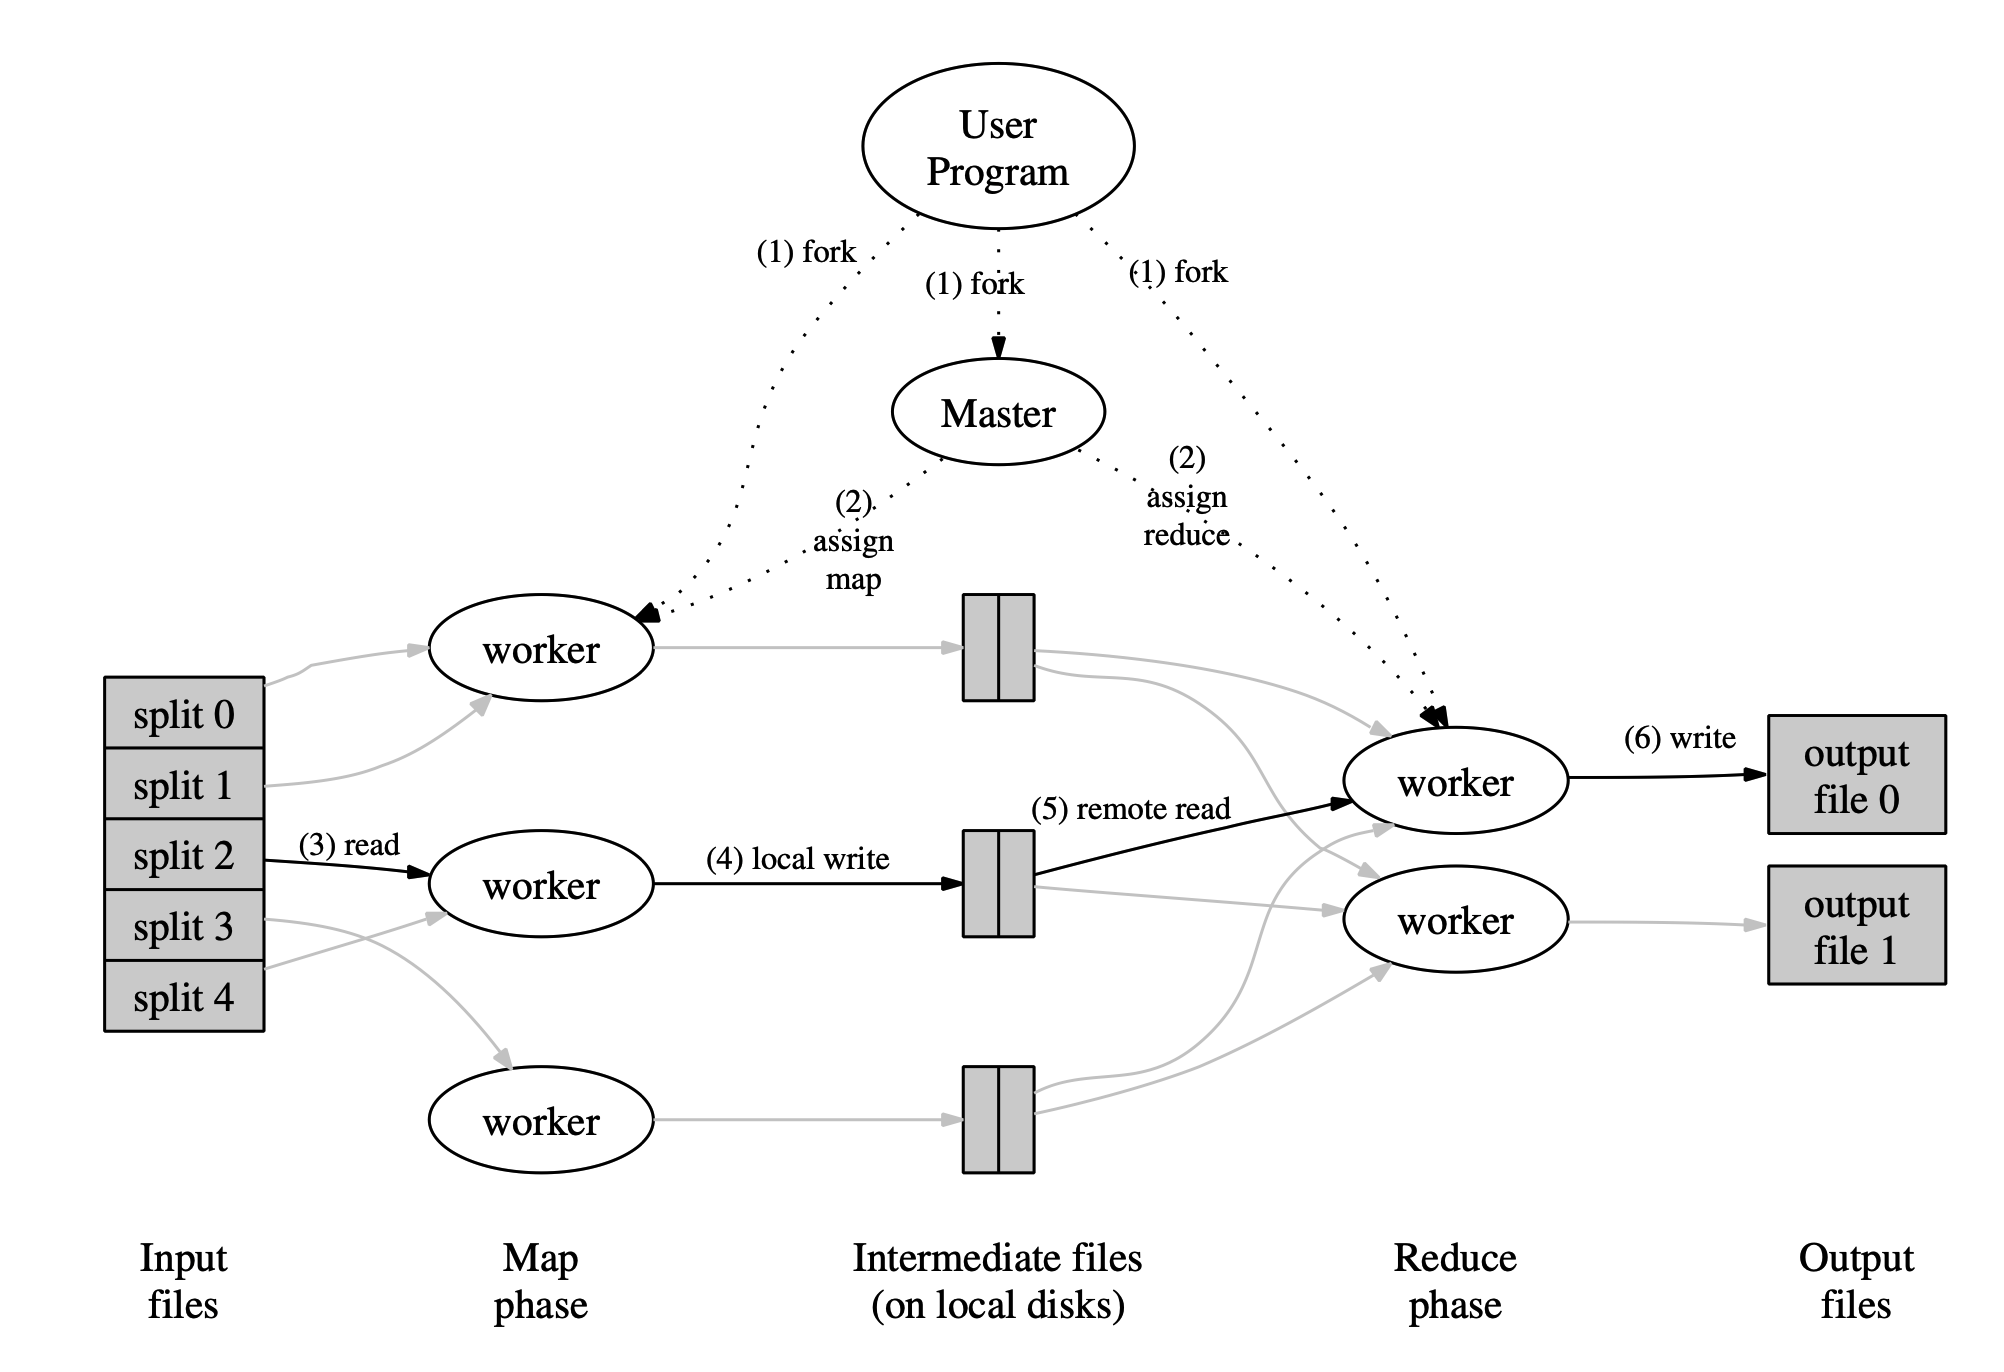
\includegraphics[width = 0.55\textwidth]{Figures/hh.png}}
	
	\begin{CJK}{UTF8}{gkai}Map worker读入1个文件,处理后生成n(reduce worker数目)个中间文件,然后每个Reduce worker读取其对应的所有中间文件,处理后生成1个结果文件,最后n个结果文件可以merge成1个最终结果文件。
	\end{CJK}
	
\end{frame}

\begin{frame}{\begin{CJK}{UTF8}{gkai}
			模块设计
	\end{CJK}}
	\begin{CJK}{UTF8}{gkai}
	主要分为Master和Worker两个模块:
	\end{CJK}
	\
	\newline\\
	
	\begin{columns}
		\begin{column}{0.5\textwidth}
			\begin{description} 
				\item[Master] 
					\begin{itemize}
						\item \begin{CJK}{UTF8}{gkai}
							对Map与Reduce任务进行切分和分配;
							
						\end{CJK}
						
						\item \begin{CJK}{UTF8}{gkai}
							当Worker无法完成任务时进行容错处理。
							
						\end{CJK}
					\end{itemize}
				
				\item[Worker] 
				\begin{itemize}
					\item \begin{CJK}{UTF8}{gkai}
						载入并执行用户设定的Map和Reduce任务;
						
					\end{CJK}
					
					\item \begin{CJK}{UTF8}{gkai}
						保存Map的中间结果并发送给Master。	
						
					\end{CJK}
				\end{itemize}
				

			\end{description}
		\end{column}
	
		\begin{column}{0.5\textwidth}
			\centerline{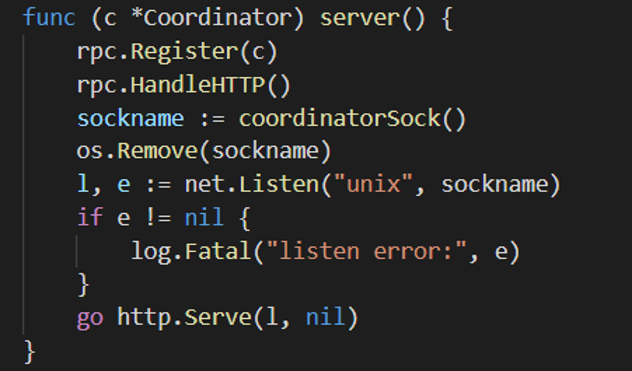
\includegraphics[width = 1.1\textwidth]{Figures/co.png}}
			\centerline{\begin{CJK}{UTF8}{gkai}两个模块之间的通信\end{CJK}
			}
		\end{column}
	\end{columns}
	
\end{frame}

\begin{frame}{\begin{CJK}{UTF8}{gkai}
			模块通信
	\end{CJK}}
	\begin{CJK}{UTF8}{gkai}
		两个模块以如下方式通信:
	\end{CJK}
	\
	\newline\\
	
	\begin{columns}
		\begin{column}{0.5\textwidth}
			\begin{description} 
				\item[Master] 
				\begin{CJK}{UTF8}{gkai}
					开启一个RPC接口,被动接受Worker的通信请求。
				\end{CJK}
				\item[Worker] 
				\begin{CJK}{UTF8}{gkai}
					通过调用Master的接口循环向Master返回执行完的任务并请求新任务。
				\end{CJK}
			\end{description}
		\end{column}
		
		\begin{column}{0.5\textwidth}
			\centerline{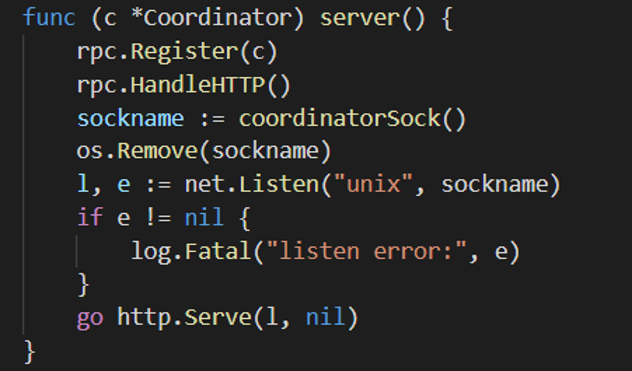
\includegraphics[width = 1.1\textwidth]{Figures/co.png}}
			\centerline{\begin{CJK}{UTF8}{gkai}两个模块之间的通信\end{CJK}
			}
		\end{column}
	\end{columns}
	
\end{frame}

\begin{frame}{\begin{CJK}{UTF8}{gkai}
			Worker结构
	\end{CJK}}
	
	\begin{columns}
		
		\begin{column}{0.5\textwidth}
			\centerline{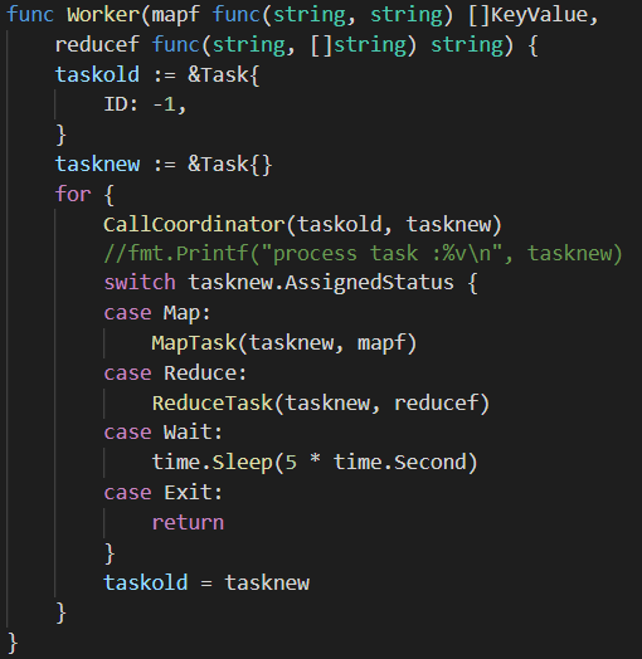
\includegraphics[width = 1.0\textwidth]{Figures/worker.png}}
		\end{column}
		\begin{column}{0.5\textwidth}
			\begin{itemize}
				\item \begin{CJK}{UTF8}{gkai}
					请求新任务;
				\end{CJK}
				
				\item \begin{CJK}{UTF8}{gkai}
					根据任务使用用户设定的Map函数或Reduce函数处理,Master暂无任务则等待;
				\end{CJK}
				
				\item \begin{CJK}{UTF8}{gkai}
					向Master返回任务执行结果并索要新任务。
				\end{CJK}	
				
			\end{itemize}
		\end{column}
		
		
	\end{columns}
	
\end{frame}

\begin{frame}{\begin{CJK}{UTF8}{gkai}
			Master结构
	\end{CJK}}
	\centerline{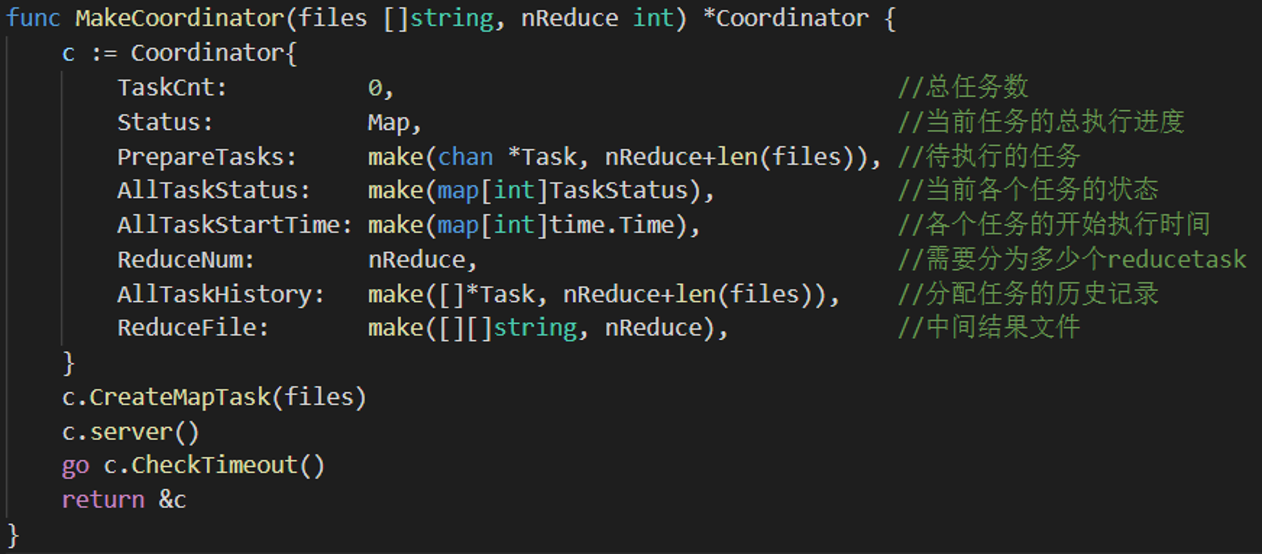
\includegraphics[width = 1.0\textwidth]{Figures/master.png}}
	\centerline{\begin{CJK}{UTF8}{gkai}
		记录总任务数,各任务状态,分配任务历史,任务执行结果。
	\end{CJK}}
	
\end{frame}

\begin{frame}{\begin{CJK}{UTF8}{gkai}
			任务创建(Master)
	\end{CJK}}
	
	\begin{columns}
		
		\begin{column}{0.5\textwidth}
			\centerline{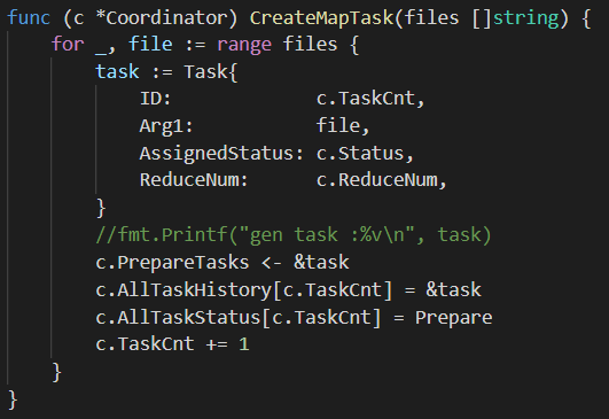
\includegraphics[width = 1.0\textwidth]{Figures/c1.png}}
			\centerline{\begin{CJK}{UTF8}{gkai}
					每个输入文件为一个Map任务。
			\end{CJK}}
		\end{column}
		
		\pause
		\begin{column}{0.5\textwidth}
			\centerline{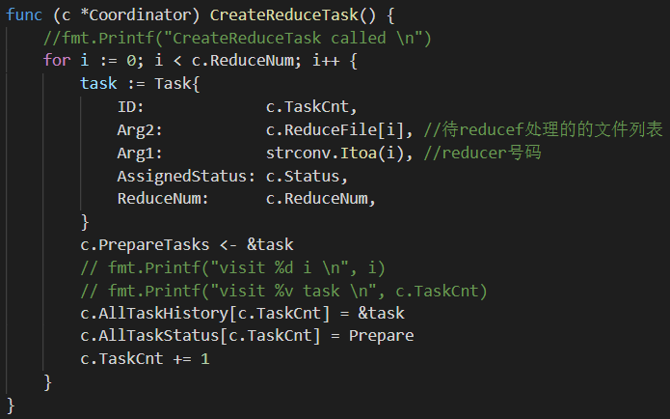
\includegraphics[width = 1.1\textwidth]{Figures/c2.png}}
			\centerline{\begin{CJK}{UTF8}{gkai}
					Reduce任务的个数手动设定。
			\end{CJK}}
		\end{column}
	\end{columns}
\end{frame}

\begin{frame}{\begin{CJK}{UTF8}{gkai}
			任务处理(Master)
	\end{CJK}}
	\centerline{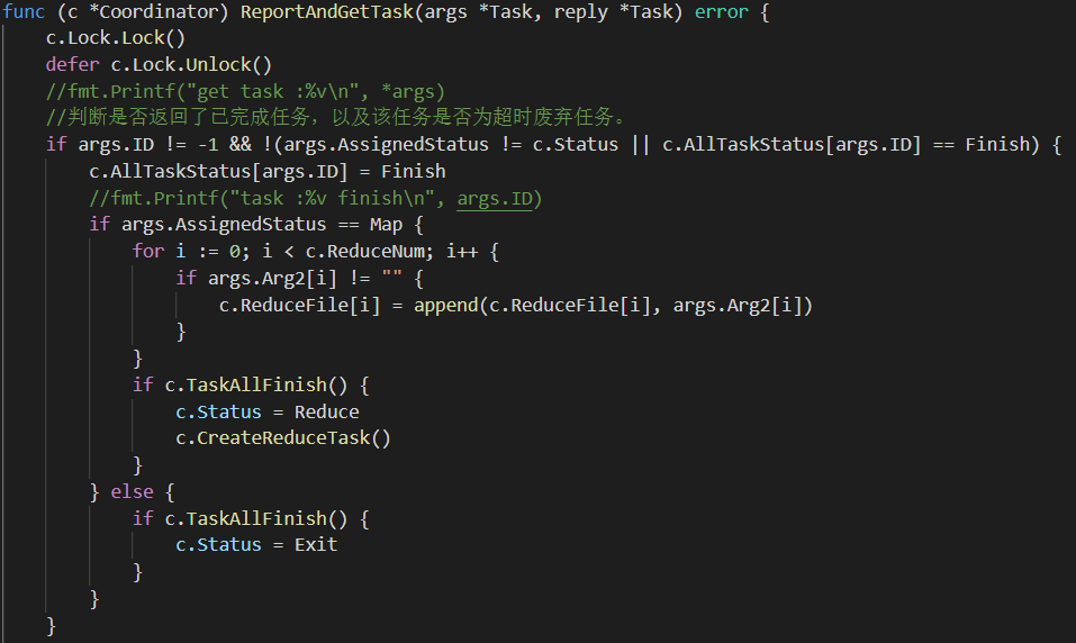
\includegraphics[width = 0.8\textwidth]{Figures/c3.png}}
	\centerline{\begin{CJK}{UTF8}{gkai}
			整理任务结果,判断是否进入下一阶段。
	\end{CJK}}
	
\end{frame}

\begin{frame}{\begin{CJK}{UTF8}{gkai}
			任务分配(Master)
	\end{CJK}}
	\centerline{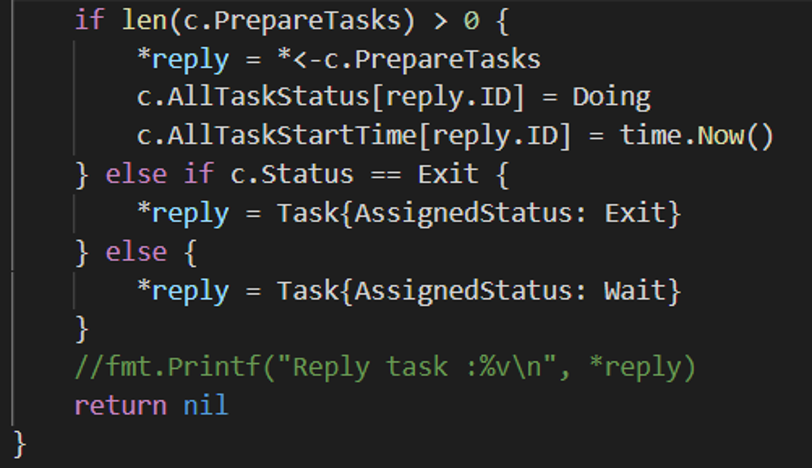
\includegraphics[width = 0.8\textwidth]{Figures/c4.png}}
	\centerline{\begin{CJK}{UTF8}{gkai}
			有任务则分配,无任务则通知Worker等待。
	\end{CJK}}
	
\end{frame}

\begin{frame}{\begin{CJK}{UTF8}{gkai}
			容错处理(Master)
	\end{CJK}}
	\centerline{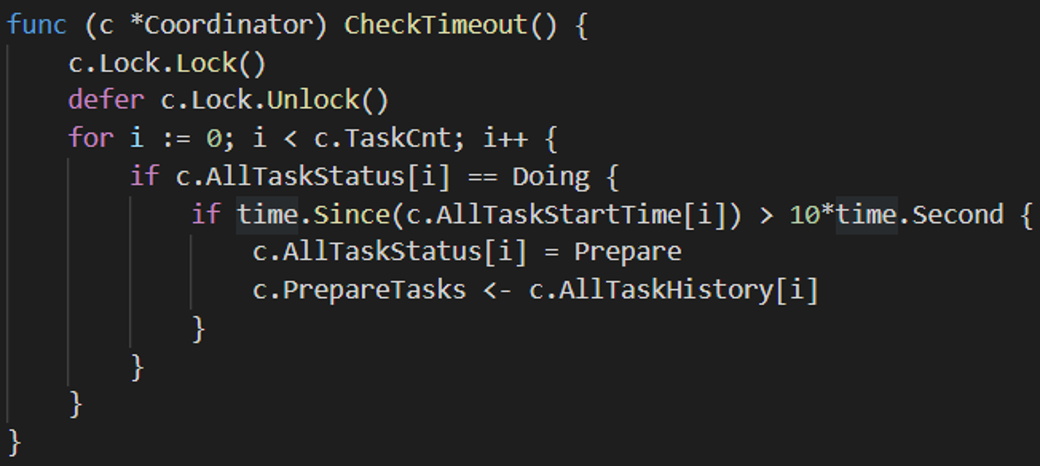
\includegraphics[width = 0.8\textwidth]{Figures/c5.png}}
	\centerline{\begin{CJK}{UTF8}{gkai}
			定期检查是否有超时仍未完成的任务,将超时任务重新改为待分配状态。
	\end{CJK}}
	
\end{frame}





\section{\begin{CJK}{UTF8}{gkai}
		MapReduce应用
\end{CJK}}

\subsection{\begin{CJK}{UTF8}{gkai}
		使用探索
\end{CJK}}

\begin{frame}{\begin{CJK}{UTF8}{gkai}
			数据文件
	\end{CJK}}
	
	\begin{columns}
		\begin{column}{0.5\textwidth}
			\begin{description} 
				\item[\begin{CJK}{UTF8}{gkai}
					数据来源
				\end{CJK}] 
				\begin{CJK}{UTF8}{gkai}
					英文名著小说等;
					
				\end{CJK}
				\item[\begin{CJK}{UTF8}{gkai}
					文件格式
				\end{CJK}] 
				\begin{CJK}{UTF8}{gkai}
					txt文本文件,前缀名统一加上pg-(方便批量处理);\\
					
				\end{CJK}
			
				\item[\begin{CJK}{UTF8}{gkai}
					文件数量
				\end{CJK}] 
				\begin{CJK}{UTF8}{gkai}
					200\\
					
				\end{CJK}
			\end{description}
		
		\centerline{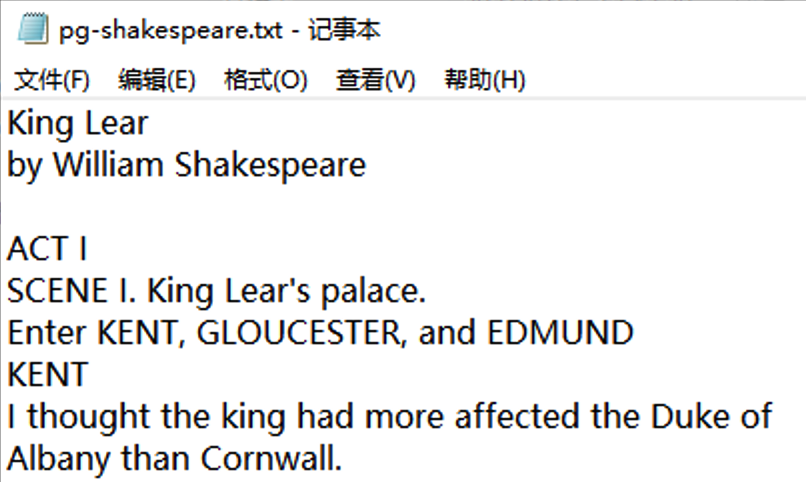
\includegraphics[width = 1.05\textwidth]{Figures/lier.png}}
		\end{column}
		
		\begin{column}{0.5\textwidth}
			\centerline{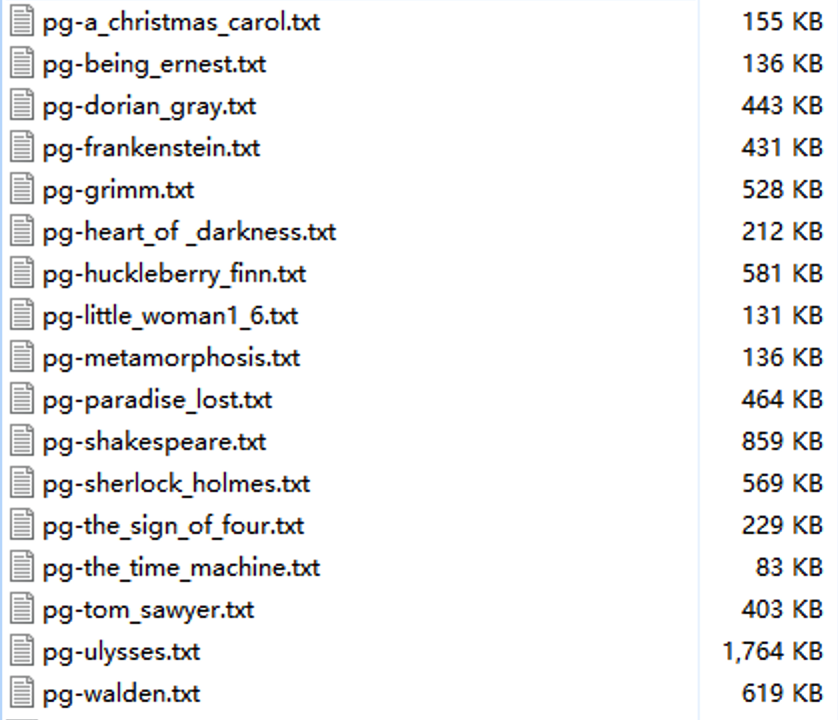
\includegraphics[width = 0.95\textwidth]{Figures/pg.png}}
			\centerline{\begin{CJK}{UTF8}{gkai}数据文件一瞥\end{CJK}
			}
		\end{column}
	\end{columns}
	
\end{frame}



\begin{frame}{Word Count}
	
	\begin{columns}
		\begin{column}{0.5\textwidth}
			\centerline{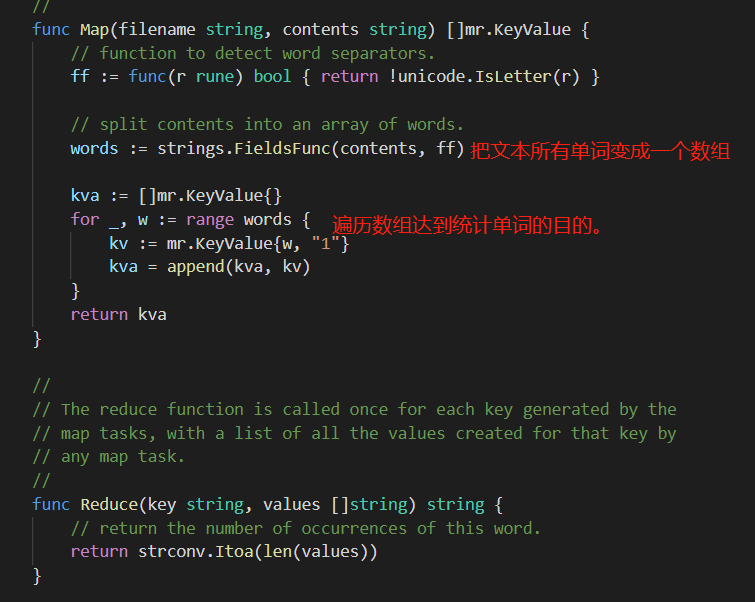
\includegraphics[width = 1.1\textwidth]{Figures/wc.png}}
			\centerline{wc.go
			}
		\end{column}
		
		\begin{column}{0.5\textwidth}
			\begin{CJK}{UTF8}{gkai}
			经典使用场景之一:词频统计
			\end{CJK}
			\begin{itemize}
				\item \begin{CJK}{UTF8}{gkai}
					先对于文件内容进行分割(strings.FieldsFunc函数);
				\end{CJK}
				
				\item \begin{CJK}{UTF8}{gkai}
					ReduceF函数接受参数为字符串切片,并对该单词的出现次数进行统计。
				\end{CJK}
				
			\end{itemize}
			\begin{block}{Word Count}
				\begin{CJK}{UTF8}{gkai}
					实现的是统计一些文档中单词出现的总次数。
				\end{CJK}
			\end{block}
		\end{column}
		
		
	\end{columns}
	
\end{frame}

\begin{frame}{Inverted index generation}
	
	\begin{columns}
		\begin{column}{0.5\textwidth}
			\centerline{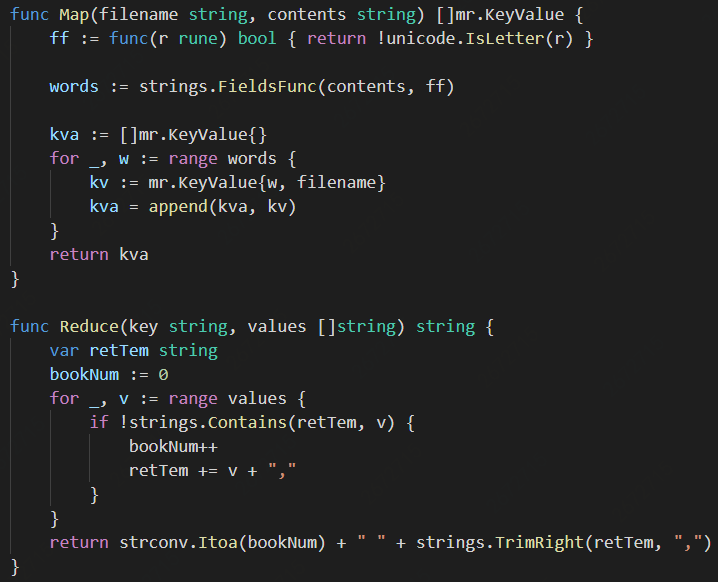
\includegraphics[width = 1.1\textwidth]{Figures/iig.png}}
			\centerline{iig.go
			}
		\end{column}
		
		\begin{column}{0.5\textwidth}
			\begin{CJK}{UTF8}{gkai}
				经典使用场景之二:反向索引
			\end{CJK}
			\begin{itemize}
				\item \begin{CJK}{UTF8}{gkai}
					Map函数与原先类似,\alert{注意生成的中间结果形式有所改变};
				\end{CJK}
				
				\item \begin{CJK}{UTF8}{gkai}
					遍历values,并分别加入到返回值中。
				\end{CJK}
				
			\end{itemize}
			\begin{block}{Inverted index generation}
				\begin{CJK}{UTF8}{gkai}
					反向索引,实现统计有单词出现的文档数。
				\end{CJK}
			\end{block}
		\end{column}
		
		
	\end{columns}
	
\end{frame}

\subsection{\begin{CJK}{UTF8}{gkai}
		并行性分析
\end{CJK}}

\begin{frame}{\begin{CJK}{UTF8}{gkai}
			试验平台
	\end{CJK}}
	
	\begin{CJK}{UTF8}{gkai}
	本次所有测试均在临湖草堂完成:
\end{CJK}
	\begin{itemize}
		\item 
		\begin{CJK}{UTF8}{gkai}
		运行命令:bash test-run.sh 10 wc pg*\end{CJK}\\
	\begin{CJK}{UTF8}{gkai}
		其中10为Worker数目,wc对应wc.go,pg*指定所处理的文件;
	\end{CJK}
	\end{itemize}

	\begin{columns}[c]
		\begin{column}{0.5\textwidth}
			\centerline{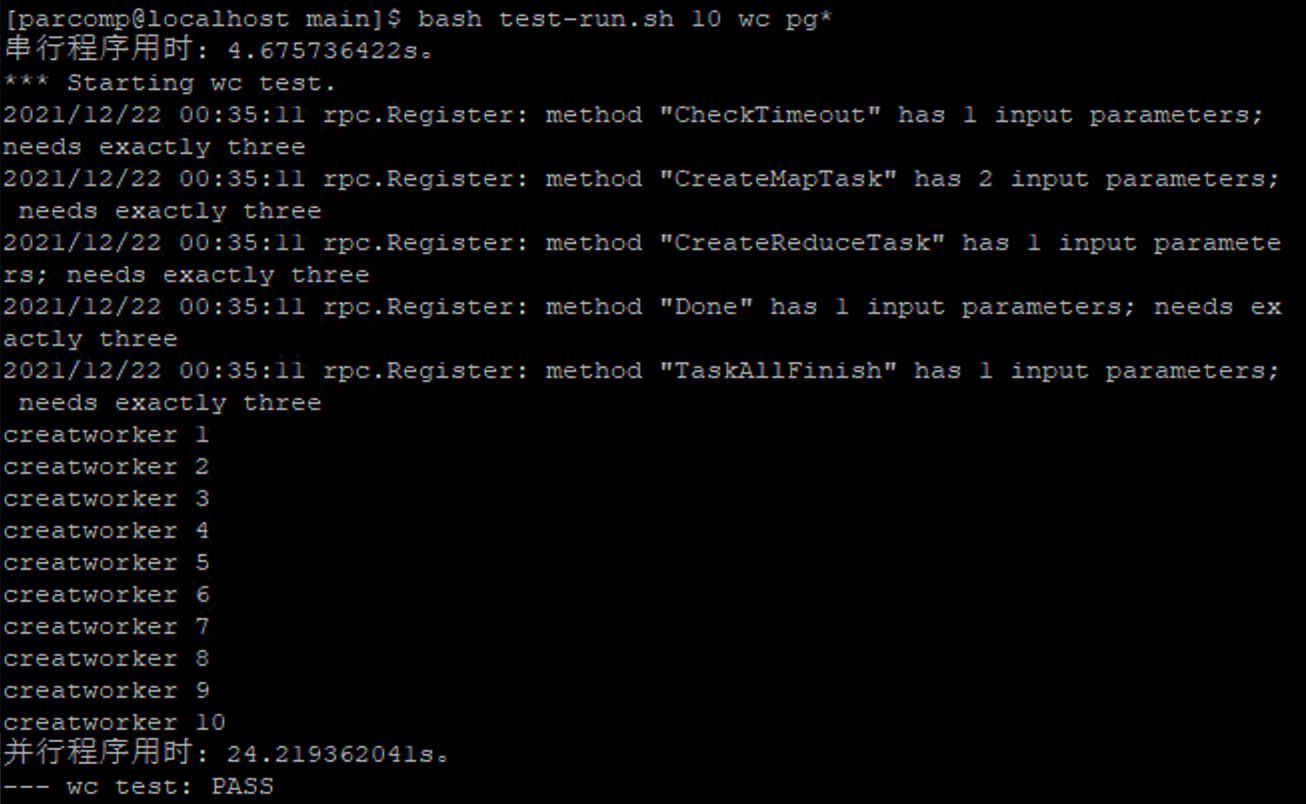
\includegraphics[width = 1.0\textwidth]{Figures/test.png}}
			\centerline{\begin{CJK}{UTF8}{gkai}运行实例\end{CJK}}
				
			\end{column}
			\vrule{}
			\begin{column}{0.5\textwidth}
				\centerline{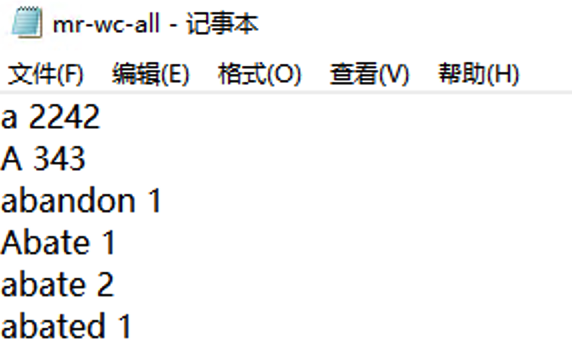
\includegraphics[width = 1.0\textwidth]{Figures/out.png}}
				\centerline{\begin{CJK}{UTF8}{gkai}并行输出文件\end{CJK}}
			\end{column}	
		\end{columns}
		
	
\end{frame}

\begin{frame}{\begin{CJK}{UTF8}{gkai}并行效果\end{CJK}}
	\begin{CJK}{UTF8}{gkai}
	我们首先考察文件规模对并行效果的影响:
\end{CJK}
		\begin{table}[ht]
			\centering
			\begin{tabular}{c || c || c || c}
	\textbf{\begin{CJK}{UTF8}{gkai}文件数目
	\end{CJK}} &\begin{CJK}{UTF8}{gkai}Worker数目
\end{CJK} &\textbf{\begin{CJK}{UTF8}{gkai}串行耗时
\end{CJK}} &\textbf{\begin{CJK}{UTF8}{gkai}并行耗时
\end{CJK}}\\
	\hline
	50 &4 &9.4s &31s\\
	\hline
	100 &4 &19.9s &56.23s\\
	\hline
	150 &4 &32s &83s\\
	\hline
	200 &4 &38.8s &106.2s\\
	
	
\end{tabular}

			%\caption{Table 1}
		\end{table}
		\begin{CJK}{UTF8}{gkai}
			\centerline{单机运行的MapReduce效果并不优于串行程序。}\\
			\
			\newline\\
			主要原因:\\
			我们保留了类似多机MapReduce的数据传输方法,导致增加了额外的运算量。
		\end{CJK}
\end{frame}

\begin{frame}{\begin{CJK}{UTF8}{gkai}并行效果\end{CJK}}
	\begin{CJK}{UTF8}{gkai}
		我们接着考察Worker数目对并行效果的影响:
	\end{CJK}
	\begin{table}[ht]
		\centering
		\begin{tabular}{c || c || c || c}
	\textbf{\begin{CJK}{UTF8}{gkai}文件数目
	\end{CJK}} &\begin{CJK}{UTF8}{gkai}Worker数目
	\end{CJK} &\textbf{\begin{CJK}{UTF8}{gkai}串行耗时
	\end{CJK}} &\textbf{\begin{CJK}{UTF8}{gkai}并行耗时
	\end{CJK}}\\
\hline
100 &2 &19.9s &104.5s\\
	\hline
	100 &3 &19.9s &70.7s\\
	\hline
	100 &4 &19.9s &56.23s\\
	\hline
	100 &5 &19.9s &48.2s\\
	
	
	
\end{tabular}
		%\caption{Table 1}
	\end{table}
	\begin{CJK}{UTF8}{gkai}
		\centerline{在单机下,Worker数目的增加的确能够提高运行效率。}\\
		\
		\newline\\
		主要原因:\\
		\\
		通过多进程创建的多个Worker充分利用了计算资源,加快了任务处理速度。
	\end{CJK}
\end{frame}

\begin{frame}{\begin{CJK}{UTF8}{gkai}
			反思与展望
	\end{CJK}}
\begin{itemize}
	\item 
	\begin{CJK}{UTF8}{gkai}
	搭建并行计算的框架是一个非常精细的过程。在搭建的过程中有很多值得探索的地方如传递值还是引用,锁的粒度等。
		\end{CJK}
	\item \begin{CJK}{UTF8}{gkai}
	通过阅读论文及相关资料,我们认为该重构MapReduce框架还可以有如下提升:
	\end{CJK}
	\begin{itemize}
		\item 
		\begin{CJK}{UTF8}{gkai}
			对文件进行进一步切分,使之变成大小一致的块,加强负载均衡。
				\end{CJK}
			\item \begin{CJK}{UTF8}{gkai}
				梳理各流程耗时,进一步提升性能。
				
			\end{CJK}
		\end{itemize}
	

\end{itemize}

\end{frame}

\begin{frame}{\begin{CJK}{UTF8}{gkai}
			评价MapReduce
	\end{CJK}}
	
	\begin{block}{Pros and cons}
		\begin{columns}[c]
			\begin{column}{0.5\textwidth}
				\begin{itemize}
					\item \begin{CJK}{UTF8}{gkai}
						优点:易于编程,具有良好的扩展性,且容错性很高。
					\end{CJK}
				
					\item \begin{CJK}{UTF8}{gkai}
						缺点:不擅长做实时计算、流式计算、DAG(有向图)计算。
					\end{CJK}
				\end{itemize}
					
			\end{column}
			\vrule{}
			\begin{column}{0.5\textwidth}
				\begin{CJK}{UTF8}{gkai}
					其他应用场景:
				\end{CJK}
				\begin{itemize}
					\item \begin{CJK}{UTF8}{gkai}
						计算URL的访问频率(Google);
					\end{CJK}
					
					
					
					\item \begin{CJK}{UTF8}{gkai}
						Top K问题,例如输出某文章中的前5个出现最频繁的词汇(Word  Count的变式)。
					\end{CJK}
				\end{itemize}
			
			\end{column}	
		\end{columns}
		
	\end{block}
	
	\cite[pp.~74--75]{Summary}\\
	\begin{CJK}{UTF8}{gkai}
	\alert{MapReduce编程模型既简单又强大},简单是因为它只包含Map和Reduce两个过程,强大之处又在于它可以实现大数据领域几乎所有的计算需求。这也正是MapReduce这个模型令人着迷的地方。
\end{CJK}
	
\end{frame}

